\documentclass[12pt]{article}

\usepackage[utf8]{inputenc}
\usepackage[english, russian]{babel}

% "А вот теперь --- слайды!"
\usepackage{slides}

% ШРИФТЫ
% Нужны рубленные шрифты -- раскомментируйте стоку ниже. 
% Нужны шрифты с засечками --- закомментируйте эту строку. 
% \renewcommand{\familydefault}{\sfdefault} % Переключает на рубленный шрифт.
% Шрифты Times и Arial, если стоит пакет cyrtimes. 
% Если он не стоит, результат будет плохой!
\usepackage{cyrtimespatched}
% Если нет cyrtimes, то попробуйте включить полужирный шрифт:
% \renewcommand{\seriesdefault}{b} % для шрифта с засечками, это предпочтительно
% \renewcommand{\seriesdefault}{sbc} % для рубленного шрифта


% Прочие пакетики
% Графика.
% Картинки и tikz
\usepackage[pdftex]{graphicx}
\usepackage{tikz}
\usepackage{pgfplots}
\pgfplotsset{compat=newest}
\usetikzlibrary{arrows,shapes,calc,decorations,chains,scopes,positioning,snakes,shadows}
\usepackage{tikz-er2}

\usepackage{amssymb}
\usepackage{amsmath}


\usepackage[underline=true,rounded corners=false]{pgf-umlsd}


\newcommand{\important}[1]{\emph{#1}}

% Настройка презентации
% Студент и руководитель.
\def\Student{Захаров Николай Игоревич}
\def\Advisor{Майков Константин Анатольевич}
% \def\Person
% \def\Affilation
% Титульный лист.
\def\Title{Программно-алгоритмический комплекс голосовой аутентификации пользователя}
\def\SubTitle{Квалификационная работа}
\newcommand{\TitleSlide}{
    \addcontentsline{toc}{section}{\Title}%
    ~\vspace{1cm}

    \begin{center}
    {\huge \begin{spacing}{1}\Title\end{spacing}}

    {\SubTitle}
    \vspace{2cm}

    \ifthenelse{\isundefined{\Student}}{}
        {\small Студент: \Student\\}
    \ifthenelse{\isundefined{\Advisor}}{}
        {\small Руководитель: \Advisor\\}
    \ifthenelse{\isundefined{\Person}}{}
        {\Person\\}
    \ifthenelse{\isundefined{\Affilation}}{}
        {\Affilation\\}
    \end{center}
    \thispagestyle{empty}
}


% Верхний заголовок: пустой
% Нижний заголовок по-умолчанию:
% \lfoot{\Title} % слева
% \cfoot{} % цент пуст
% \rfoot{\thepage} % справа

% \renewcommand{\baselinestretch}{1.5}
% \linespread{1.6}

\begin{document}

\TitleSlide

% Команды section и section начинают новый слайд.

\section{Цель и задачи работы}

Создание программно-алгоритмического комплекса голосовой аутентификации пользователя.

\begin{enumerate}
\item Проанализировать существующие решения в области голосовой аутентификации;
\item Разработать программно-аппаратный комплекс, позволяющий принимать, обрабатывать голосовые данные, а также принимать решение об аутентификации;
\item Разработать схему хранения голосовых данных на сервере;
\item Обеспечить работу системы в условиях мультиплатформенной программно-аппаратной среды;
\item Исследовать разработанный программный комплекс, оценить его работоспособность.
\end{enumerate}

\section{Задача голосовой верификации}

Проверка статистической гипотезы для источника речи $S$:

\begin{equation}
\label{eq:hypothesis}
\left\{ 
    \begin{array}{lll}
        H_0 & : & \textrm{высказывание } X \textrm{ произнес } S;\\
        H_1 & : & \textrm{высказывание } X \textrm{ произнес \important{не} } S.\\
    \end{array}
\right.
\end{equation}

\section{Основные этапы работы системы голосовой аутентификации}

\begin{enumerate}
\item Нормализация входного речевого сигнала;
\item Выделение характерных признаков;
\item Построение модели источника речи (стадия обучения);
\item Принятие по построенной модели и новой входной последовательности одной из двух гипотез (\ref{eq:hypothesis}).
\end{enumerate}

\section{Диаграмма функциональных блоков процесса верификации}

\begin{figure}[h!]
\center{\includegraphics[width=\textwidth]{../include/idef0_main_dia}}
\end{figure}

\section{Нормализация речевого сигнала}

\begin{itemize}
    \item удаление тишины;
    \item частотная развертка (учет ограниченности спектра человеческой речи);
    \item нормализация по средним (\important{mean normalization});
\end{itemize}

\section{Выделение характерных признаков}

Преобразование сегментированного сигнала в массив векторов характерных признаков:
\begin{itemize}
    \item коэффициенты кода линейного предсказания (\important{LPCС});
    \item коэффициенты Вейвлет-преобразования;
    \item мел-частотные коэффициенты кепстра (\important{MFCC}).
\end{itemize}

\section{Диаграмма функциональных блоков обработки речи}

\begin{figure}[h!]
\center{\includegraphics[width=\textwidth]{../include/idef0_pre_dia}}
\end{figure}

\section{Подходы к моделированию источника речи}

\begin{itemize}
\item алгоритмы сопоставления с образцом: динамического временного преобразования (\emph{DTW}), Евклидово расстояние, расстояние Махаланобиса.
\item скрытые Марковские модели (\emph{HMM}, \emph{Hidden Markov Models});
\item искусственные нейронные сети;
\item смеси Гауссиан (\emph{GMM}, \emph{Gaussian Mixture Models}).
\end{itemize}

\section{Модели на основе смеси Гауссиан}

Моделируем плотность распределения вектора характерных признаков через взвешенную сумму $K$ нормальных распределений:

\begin{equation}
p(\vec x | \lambda) = \sum_{i=1}^K{\omega_i p_i(\vec x)},
\end{equation}

\noindent где $K$ -- количество компонент,\\
$\vec x$ -- вектор характерных признаков,\\
$\omega_i$ -- вес $i$-ой компоненты, \\
$p_i$ -- плотность распределения $i$-ой компоненты.

\section{Пример моделирования распределения с помощью смеси Гауссиан}

\begin{figure}[h!]
\center{\includegraphics[height=.75\textheight]{../include/gmm_merged_full_svg}}
\end{figure}

\section{Проблемы при использовании смеси Гауссиан}

\begin{itemize}
\item выбор количества компонент смеси;
\item инициализация параметров модели перед обучением;
\item исчезновение порядка в матрице ковариаций;
\item вычисление правдоподобия альтернативной гипотезы:
    \begin{itemize}
        \item универсальная фоновая модель: обучение GMM по нескольким часам речевых данных, сбалансированных по гендерному типу, возрасту, типу окружения;
        \item модели когортов: нахождение моделей, близких по мере правдоподобия $p(X|H_0)$ к модели целевого источника речи.
    \end{itemize}
\end{itemize}


\section{Принятие решения}

Предположим, что меры правдоподобия обеих гипотез (\ref{eq:hypothesis}) известны. Рассмотрим \important{отношение правдоподобия}:

\begin{equation}
\label{eq:lr}
LR_{H_0, H_1} = \frac{p(X|H_0)}{p(X|H_1)},
\end{equation}

\begin{equation}
\label{eq:decision}
\textrm{Решение } = \left\{ 
    \begin{array}{ll}
        H_0, & LR_{H_0, H_1} > \Theta_{S} \\
        H_1, & LR_{H_0, H_1} \leq \Theta_{S}, \\
    \end{array}
\right.
\end{equation}

\noindent где $\Theta_{S}$ -- величина порога вхождения.

\section{Общая архитектура комплекса}

\begin{figure}[h!]
\center{\includegraphics[height=.8\textheight]{../include/main_arch_dia}}
\end{figure}


\section{Диаграмма вариантов использования}

\begin{figure}[h!]
\center{\includegraphics[height=.8\textheight]{../include/use_cases_dia}}
\end{figure}

\section{Диаграмма сущность-связь системы хранения}

\begin{figure}[h!]
\center{\includegraphics[height=.79\textheight]{../include/er_main_tex}}
\end{figure}

\section{Диаграмма состояний для процесса регистрации в системе}

\begin{figure}[h!]
\center{\includegraphics[height=.8\textheight]{../include/enrollment_server_sd_dia}}
\end{figure}

\section{Диаграмма последовательности для процесса аутентификации}
\begin{figure}[hp!]
    \center{
        \includegraphics[height=0.78\textheight]{../include/seq_enrollment_tex}
    }
\end{figure}

\section{Блок-схема алгоритма удаления тишины из входного сигнала}
 
\begin{figure}[htp!]
    \center{
    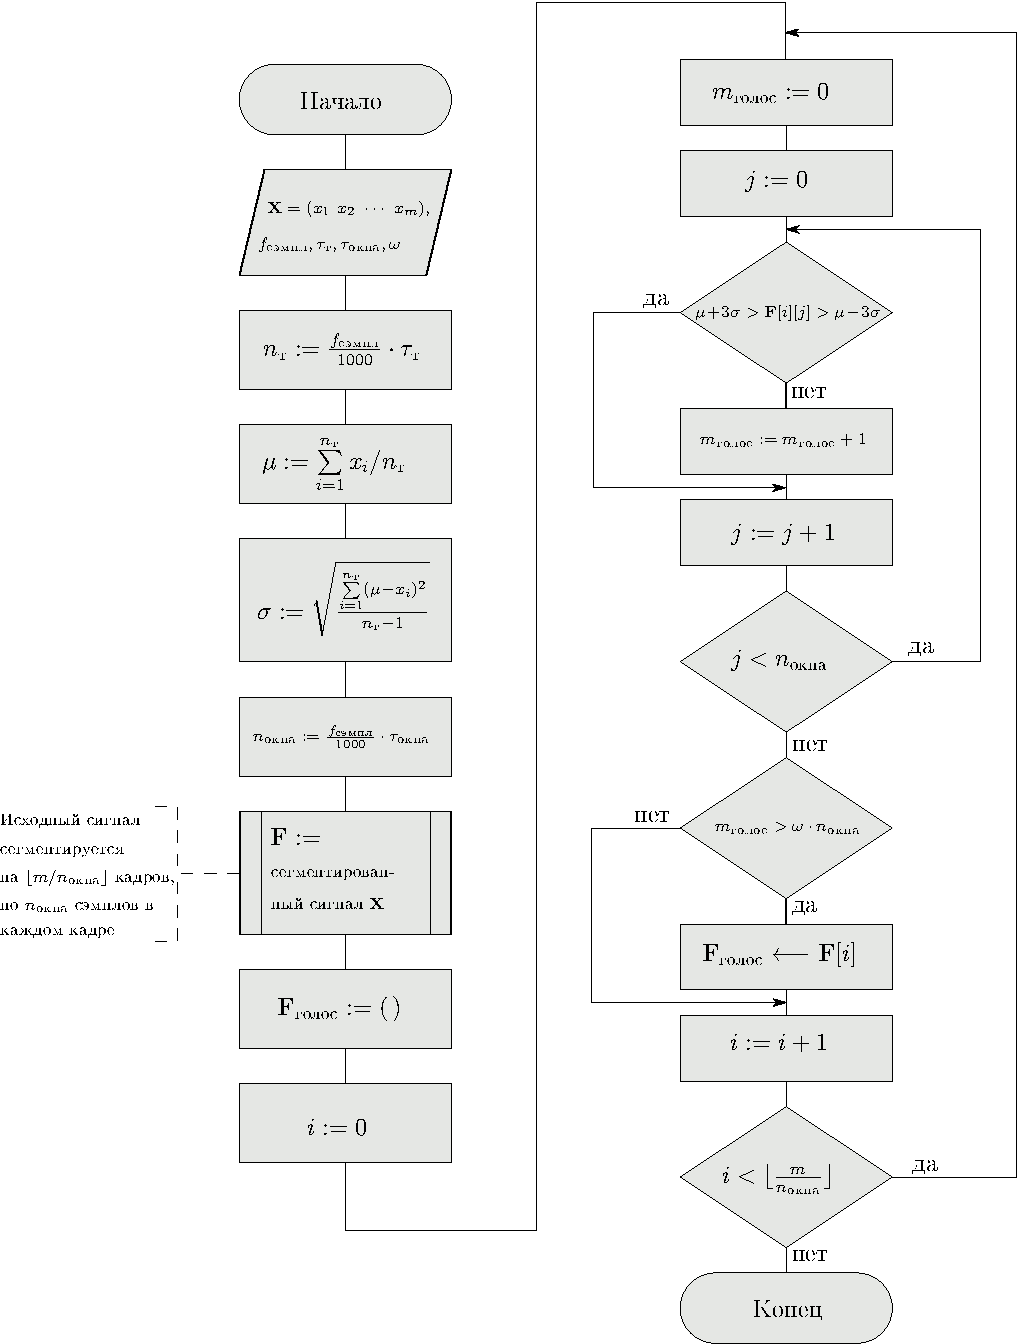
\includegraphics[height=0.78\textheight]{../static_include/silence_remove_flowchart}
    }
\end{figure}


\section{Исследование показателей качества программного комплекса}

В качестве характеристик качества аутентификации принимаются вероятности совершения ошибок I-ого и II-ого рода:
\begin{enumerate}
\item Аутентификация завершилась неудачно для аутентичного источника речи (ложный отрицательный);
\item Аутентификация прошла успешно, но источник речи в действительности не аутентичен зарегистрированному (несанкционированный вход, ложный положительный).
\end{enumerate}

Требуемый баланс между этими показателями достигается путем варьирования значения порога вхождения.
Частота равнозначной ошибки (\important{Equal Error Rate})~--- значение вероятности при таком пороге вхождения, при котором вероятности ошибок I-ого и II-ого рода равны.

\section{Зависимость частоты равнозначной ошибки от количества компонент модели}
\begin{figure}[hp!]
    \center{
        \includegraphics[height=0.75\textheight]{../static_include/eer_from_k.pdf}
    }
\end{figure}

\section{Зависимость частоты равнозначной ошибки от количества фраз, используемых для обучения}
\begin{figure}[hp!]
    \center{
        \includegraphics[height=0.75\textheight]{../static_include/eer_from_n.pdf}
    }
\end{figure}

\section{Зависимость ошибок аутентификации от значения порога вхождения}

\begin{figure}[ht!]
\center{\includegraphics[height=0.75\textheight]{../static_include/overall}}
\end{figure}



\end{document}

